%----------------------------------------------------------------------------------------
%	PACKAGES AND OTHER DOCUMENT CONFIGURATIONS
%----------------------------------------------------------------------------------------

\documentclass{article}

\usepackage{fancyhdr} % Required for custom headers
\usepackage{lastpage} % Required to determine the last page for the footer
\usepackage{extramarks} % Required for headers and footers
\usepackage[usenames,dvipsnames]{color} % Required for custom colors
\usepackage{graphicx} % Required to insert images
\usepackage{listings} % Required for insertion of code
\usepackage{courier} % Required for the courier font
\usepackage{lipsum} % Used for inserting dummy 'Lorem ipsum' text into the template
\usepackage[utf8]{inputenc}
\usepackage[ngerman]{babel}

% Margins
\topmargin=-0.45in
\evensidemargin=0in
\oddsidemargin=0in
\textwidth=6.5in
\textheight=9.0in
\headsep=0.25in

\linespread{1.1} % Line spacing

% Set up the header and footer
\pagestyle{fancy}
%\lhead{\hmwkAuthorName} % Top left header
\chead{\hmwkClass\ : \hmwkTitle} % Top center head
\rhead{\firstxmark} % Top right header
\lfoot{\lastxmark} % Bottom left footer
\cfoot{} % Bottom center footer
\rfoot{Page\ \thepage\ of\ \protect\pageref{LastPage}} % Bottom right footer
\renewcommand\headrulewidth{0.4pt} % Size of the header rule
\renewcommand\footrulewidth{0.4pt} % Size of the footer rule

\setlength\parindent{0pt} % Removes all indentation from paragraphs

%----------------------------------------------------------------------------------------
%	CODE INCLUSION CONFIGURATION
%----------------------------------------------------------------------------------------

\definecolor{MyDarkGreen}{rgb}{0.0,0.4,0.0} % This is the color used for comments
\lstloadlanguages{Perl} % Load Perl syntax for listings, for a list of other languages supported see: ftp://ftp.tex.ac.uk/tex-archive/macros/latex/contrib/listings/listings.pdf
\lstset{language=Perl, % Use Perl in this example
        frame=single, % Single frame around code
        basicstyle=\small\ttfamily, % Use small true type font
        keywordstyle=[1]\color{Blue}\bf, % Perl functions bold and blue
        keywordstyle=[2]\color{Purple}, % Perl function arguments purple
        keywordstyle=[3]\color{Blue}\underbar, % Custom functions underlined and blue
        identifierstyle=, % Nothing special about identifiers                                         
        commentstyle=\usefont{T1}{pcr}{m}{sl}\color{MyDarkGreen}\small, % Comments small dark green courier font
        stringstyle=\color{Purple}, % Strings are purple
        showstringspaces=false, % Don't put marks in string spaces
        tabsize=5, % 5 spaces per tab
        %
        % Put standard Perl functions not included in the default language here
        morekeywords={rand},
        %
        % Put Perl function parameters here
        morekeywords=[2]{on, off, interp},
        %
        % Put user defined functions here
        morekeywords=[3]{test},
       	%
        morecomment=[l][\color{Blue}]{...}, % Line continuation (...) like blue comment
        numbers=left, % Line numbers on left
        firstnumber=1, % Line numbers start with line 1
        numberstyle=\tiny\color{Blue}, % Line numbers are blue and small
        stepnumber=5 % Line numbers go in steps of 5
}

% Creates a new command to include a perl script, the first parameter is the filename of the script (without .pl), the second parameter is the caption
\newcommand{\perlscript}[2]{
\begin{itemize}
\item[]\lstinputlisting[caption=#2,label=#1]{#1.pl}
\end{itemize}
}

%----------------------------------------------------------------------------------------
%	DOCUMENT STRUCTURE COMMANDS
%	Skip this unless you know what you're doing
%----------------------------------------------------------------------------------------

% Header and footer for when a page split occurs within a problem environment
\newcommand{\enterProblemHeader}[1]{
%\nobreak\extramarks{#1}{#1 continued on next page\ldots}\nobreak
%\nobreak\extramarks{#1 (continued)}{#1 continued on next page\ldots}\nobreak
}

% Header and footer for when a page split occurs between problem environments
\newcommand{\exitProblemHeader}[1]{
%\nobreak\extramarks{#1 (continued)}{#1 continued on next page\ldots}\nobreak
%\nobreak\extramarks{#1}{}\nobreak
}

\setcounter{secnumdepth}{0} % Removes default section numbers
\newcounter{homeworkProblemCounter} % Creates a counter to keep track of the number of problems

\newcommand{\homeworkProblemName}{}
\newenvironment{homeworkProblem}[1][Problem \arabic{homeworkProblemCounter}]{ % Makes a new environment called homeworkProblem which takes 1 argument (custom name) but the default is "Problem #"
\stepcounter{homeworkProblemCounter} % Increase counter for number of problems
\renewcommand{\homeworkProblemName}{#1} % Assign \homeworkProblemName the name of the problem
\section{\homeworkProblemName} % Make a section in the document with the custom problem count
%\enterProblemHeader{\homeworkProblemName} % Header and footer within the environment
}{
%\exitProblemHeader{\homeworkProblemName} % Header and footer after the environment
}

\newcommand{\problemAnswer}[1]{ % Defines the problem answer command with the content as the only argument
\noindent\framebox[\columnwidth][c]{\begin{minipage}{0.98\columnwidth}#1\end{minipage}} % Makes the box around the problem answer and puts the content inside
}

\newcommand{\homeworkSectionName}{}
\newenvironment{homeworkSection}[1]{ % New environment for sections within homework problems, takes 1 argument - the name of the section
\renewcommand{\homeworkSectionName}{#1} % Assign \homeworkSectionName to the name of the section from the environment argument
\subsection{\homeworkSectionName} % Make a subsection with the custom name of the subsection
%\enterProblemHeader{\homeworkProblemName\ [\homeworkSectionName]} % Header and footer within the environment
}{
%\enterProblemHeader{\homeworkProblemName} % Header and footer after the environment
}

%----------------------------------------------------------------------------------------
%	NAME AND CLASS SECTION
%----------------------------------------------------------------------------------------

\newcommand{\hmwkTitle}{Übung\ \#2} % Assignment title
\newcommand{\hmwkDueDate}{Donnerstag,\ 06.\ November\ 2014} % Due date
\newcommand{\hmwkClass}{GPU Computing} % Course/class
\newcommand{\hmwkClassTime}{} % Class/lecture time
\newcommand{\hmwkClassInstructor}{} % Teacher/lecturer
\newcommand{\hmwkAuthorName}{Günther Schindler, Alexander Schapp, Klaus Naumann} % Your name

%----------------------------------------------------------------------------------------
%	TITLE PAGE
%----------------------------------------------------------------------------------------

\title{
\vspace{2in}
\textmd{\textbf{\hmwkClass:\ \hmwkTitle}}\\
\normalsize\vspace{0.1in}\small{Abgabe\ am\ \hmwkDueDate}\\
\vspace{0.1in}\large{\textit{\hmwkClassTime}}
\vspace{3in}
}

\author{\textbf{\hmwkAuthorName}}
\date{} % Insert date here if you want it to appear below your name

%----------------------------------------------------------------------------------------

\begin{document}

\maketitle

%----------------------------------------------------------------------------------------
%	TABLE OF CONTENTS
%----------------------------------------------------------------------------------------

%\setcounter{tocdepth}{1} % Uncomment this line if you don't want subsections listed in the ToC

\newpage
\tableofcontents
\newpage

%----------------------------------------------------------------------------------------
%	Raw Kernel Startup Time
%----------------------------------------------------------------------------------------

% To have just one problem per page, simply put a \clearpage after each problem

\begin{homeworkProblem}[Raw Kernel Startup Time]
In der ersten Aufgabenstellung ging es darum die \textit{Startup} Zeiten für synchrone und asynchrone Kernelstartvorgänge zu messen. Dies sollte unter der Variation von \textit{thread blocks} und \textit{threads per block} durchgeführt werden. Der Wertebereich is hierbei von 1 bis 1024 für beide Parameter vorgegeben.\\ \\
Ausgangspunkt war die zur Verfügung gestellte Datei \textit{nullKernelAsynch.cu}, welche asychrone Kernelstartvorgänge misst. Um die synchronen Kernelstartvorgänge zu messen wurde eine zweite Datei \textit{nullKernelSynch.cu} erstellt. \\ \\
Auszug aus \textit{nullKernelAsynch.cu}:
\begin{lstlisting}{c}
    chTimerGetTime( &start );
    for ( int i = 0; i < cIterations; i++ ) {
        NullKernel<<<1,1>>>();
    }
    cudaThreadSynchronize();
    chTimerGetTime( &stop );
\end{lstlisting}
Hier findet die Synchronisation erst statt, nachdem die for-Schleife verlassen wird. Solange die Schleife läuft, wird bei jedem Iterationsschritt i ein neuer Kernel gestartet, unabhängig davon ob der Kernel, der zum Iterationsschritt i - 1 gestartet wurde, seine Berechnungen bereits abgeschlossen hat.  \\ 

Um die synchronen Startvorgänge zu messen musste der oben dargestellte Code, für \textit{nullKernelSynch.cu}, wie folgt abgeändert werden:
\begin{lstlisting}{c}
    chTimerGetTime( &start );
    for ( int i = 0; i < cIterations; i++ ) {
        NullKernel<<<1,1>>>();
        cudaThreadSynchronize();
    }
    chTimerGetTime( &stop );
\end{lstlisting}
Bei diesem Code wird nach jedem Kernelstart, innerhalb der Schleife, eine Synchronisation ausgeführt. Dies führt dazu, dass ein neuer Kernel erst dann gestartet wird, wenn der aktuelle Kernel seine Berechnungen abgeschlossen hat. \\

Für die asynchrone Variante wurden folgende Werte gemessen: \\ \\
\begin{tabular}{|c|c|c|}
\hline
	thread blocks & threads per block & time in micros\\
\hline
	1024 & 1 & 1.97\\
\hline
	512 & 2 & 1.95\\
\hline
	256 & 4 & 1.94\\
\hline
	128 & 8 & 1.92\\
\hline
	64 & 16 & 1.92\\
\hline
	32 & 32 & 1.88\\
\hline
	16 & 64 & 1.95\\
\hline
	8 & 128 & 1.85\\
\hline
	4 & 256 & 1.93\\
\hline
	2 & 512 & 1.92\\
\hline
\end{tabular}
\begin{tabular}{|c|c|c|}
\hline
	thread blocks & threads per block & time in micros\\
\hline
	1 & 1024 & 1.93\\
\hline
	1 & 512 & 1.90\\
\hline
	1 & 256 & 1.92\\
\hline
	1 & 128 & 1.90\\
\hline
	1 & 64 & 1.91\\
\hline
	1 & 32 & 1.93\\
\hline
	1 & 16 & 1.89\\
\hline
	1 & 8 & 1.94\\
\hline
	1 & 4 & 1.97\\
\hline
	1 & 2 & 1.95\\
\hline
\end{tabular}
\\ \\ \\ \\
Für die synchrone Variante wurden folgende Werte gemessen: \\ \\
\begin{tabular}{|c|c|c|}
\hline
	thread blocks & threads per block & time in micros\\
\hline
	1024 & 1 & 9.29\\
\hline
	512 & 2 & 7.91\\
\hline
	256 & 4 & 7.11\\
\hline
	128 & 8 & 6.65\\
\hline
	64 & 16 & 6.43\\
\hline
	32 & 32 & 6.44\\
\hline
	16 & 64 & 6.47\\
\hline
	8 & 128 & 6.51\\
\hline
	4 & 256 & 6.49\\
\hline
	2 & 512 & 6.45\\
\hline
\end{tabular}
\begin{tabular}{|c|c|c|}
\hline
	thread blocks & threads per block & time in micros\\
\hline
	1 & 1024 & 6.69\\
\hline
	1 & 512 & 6.35\\
\hline
	1 & 256 & 6.70\\
\hline
	1 & 128 & 6.54\\
\hline
	1 & 64 & 6.60\\
\hline
	1 & 32 & 6.79\\
\hline
	1 & 16 & 6.75\\
\hline
	1 & 8 & 6.63\\
\hline
	1 & 4 & 6.57\\
\hline
	1 & 2 & 6.45\\
\hline
\end{tabular}
\\ \\ \\
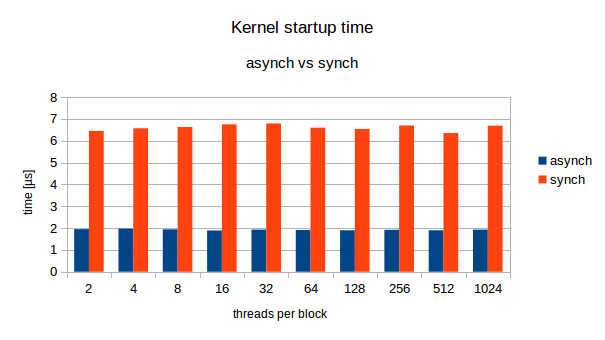
\includegraphics[width=\textwidth]{measurements.png}
Betrachtet man das Diagramm \textit{Kernel startup time} sieht man, das die durchschnittlichen Ausführungszeiten für beide Varianten eine Differenz aufweisen. Die Ausführungszeiten für die synchronisierte Variante sind im Durchschnitt etwa um den Faktor 3 länger. Betrachtet man den Code des Kernels, so stellt man fest, dass dieser leer ist.
\\
\begin{lstlisting}{c}
   	__global__
	void
	NullKernel()
	{
	}
\end{lstlisting}

Verwunderlich ist, dass obwohl im Kernel keine Berechnungen durchgeführt werden, die \textit{threads} der asynchronen Variante durchschnittlich 2 Mikrosekunden für den \textit{startup} benötigen. Es ist anzunehmen, dass die \textit{threads} diese Zeit im Treiber verbringen. Die Differenz der beiden Methoden ist demnach auf die Synchronisation zurück zu führen.



\end{homeworkProblem}
%----------------------------------------------------------------------------------------
%	Break-even Kernel Startup Time
%----------------------------------------------------------------------------------------
\begin{homeworkProblem}[Break-even Kernel Startup Time]
Hier ist ein Ausschnitt aus der Datei \textit{busywaitKernelAsync.cu}
\begin{lstlisting}{c}

__device__ int dTime;

__global__
void
busywaitKernel( int cycles, bool flag )
{
	int stop, start = clock();

	do {
		stop = clock();
	} while (stop-start < cycles);
	
	if( flag && threadIdx.x == 0 && blockIdx.x == 0 ) {
		dTime = stop - start;
	}
}

int
main( int argc, char *argv[] )
{
	const int cIterations = 1000000; 
		
    printf( "Measuring break-even kernel startup time... " ); fflush( stdout );

    chTimerTimestamp start, stop;
	
	for( int cycles = 0; cycles < 5000; cycles += 100 ) {
		printf( "Cycles: %d \n", cycles); fflush( stdout );		
    		chTimerGetTime(&start);
    		for ( int i = 0; i < cIterations; i++ ) {
        		busywaitKernel<<<1,1>>>(cycles, false);
    		}
    		cudaThreadSynchronize();
    		chTimerGetTime(&stop);	

        	double microseconds = 1e6*chTimerElapsedTime( &start, &stop );
        	double usPerLaunch = microseconds / (float) cIterations;
        	printf( "%.2f us\n", usPerLaunch );
   	}
\end{lstlisting}

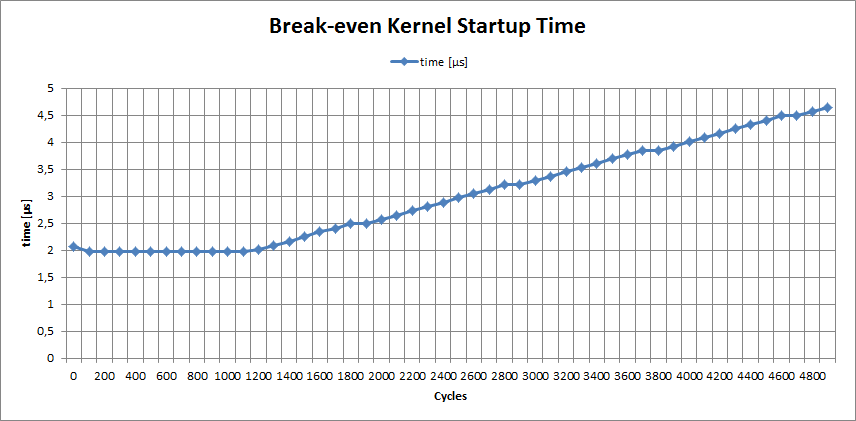
\includegraphics[width=\textwidth]{break-even.png}
\\
Im zweiten Teil der Aufgabe geht es um die \textit{Break-even Kernel Startup Time} und wie lange es dauert diese zu erreichen. Im Liniendiagramm sieht man, dass der Prozess bei 2 Mikrosekunden startet. Der Break-even wird hier bei etwa 4000 Zyklen erreicht. 

\end{homeworkProblem}

\end{document}
